\documentclass{article}
\usepackage[paperletter]{geometry}
\geometry{top=1.0in, bottom=1.0in, left=1.0in, right=1.0in}
\usepackage[utf8]{inputenc}
\usepackage{cancel}
\usepackage{tikz}
\usepackage{siunitx}
\usepackage{amsmath}
\usepackage{mathdots}
\usepackage{yhmath}
\usepackage{color}
\usepackage{array}
\usepackage{multirow}
\usepackage{amssymb}
\usepackage{gensymb}
\usepackage{tabularx}
\usepackage{booktabs}
\usepackage[symbol]{footmisc}
\renewcommand*{\thefootnote}{\fnsymbol{footnote}}
\usepackage{everysel}
\usepackage{ragged2e}
\renewcommand*\familydefault{\ttdefault}
\EverySelectfont{%
\fontdimen2\font=0.4em% interword space
\fontdimen3\font=0.2em% interword stretch
\fontdimen4\font=0.1em% interword shrink
\fontdimen7\font=0.1em% extra space
\hyphenchar\font=`\-% to allow hyphenation
}

\title{Rotational Motion \& Angular Momentum Lab \\ AP \textsc{Physics} $-$ 1}
\author{Michael \textsc{Brodskiy}}
\date{February 11, 2020}

\begin{document}

\maketitle
\begin{center}
\begin{tabular}{l r}
\underline{Date Performed}: & February 6, 2020 \\\\ % Date the experiment was performed
\underline{Partners}: & McKenna Dixon \\ & Graham Horrigan \\ & Ryan Jacoby \\\\
\underline{Instructor}: & Mrs. Halle \\\\\\\\\\ % Instructor/supervisor
\end{tabular}
\end{center}
\newpage

\begin{center}
\section{Pre-Lab Questions}
\end{center}

\vspace{24pt}
\flushleft{1. A .15[\si{\kilogram}] block is held 1[\si{\meter}] above the floor. Calculate the time it will take for the object to strike the ground.\\
\textit{**free fall problem**}}

\centering{By using the equation:}
$$ \Delta x = v_{oy}t + \frac{1}{2}a_yt^2$$
\centering{ We get:}
$$ -1 = \frac{1}{2}gt^2$$
\centering {Once $t$ is solved for, we find:}
$$ t = .451[\si{\second}]$$

\newpage
\flushleft{2. Consider the same block hanging vertically and attached by a cord and pulley to a .1[\si{\gram}] frictionless cart sitting on a table. Calculate the time it takes for the object to strike the ground once it is released.\\
\vspace{24pt}
\textit{**atwood machine problem**}}
\vspace{92pt}

\begin{figure}[ht]
\begin{minipage}[b]{0.45\linewidth}
\vspace{36pt}
By using the equation:
$$g(m_2-m_1) = (m_1+m_2)a$$ 
We get:
$$g(.15-.0001) = (.15+.0001)a$$
Then, $a$ is found to be:
$$a = 9.8001$$
This can then be used to find $t$:
$$t = \sqrt{\frac{2}{a}} = .4518[\si{\second}]$$
\vspace{36pt}
\end{minipage}
\hfill\vline\hfill
\begin{minipage}[b]{0.45\linewidth}
\centering
\tikzset{every picture/.style={line width=0.75pt}} %set default line width to 0.75pt        

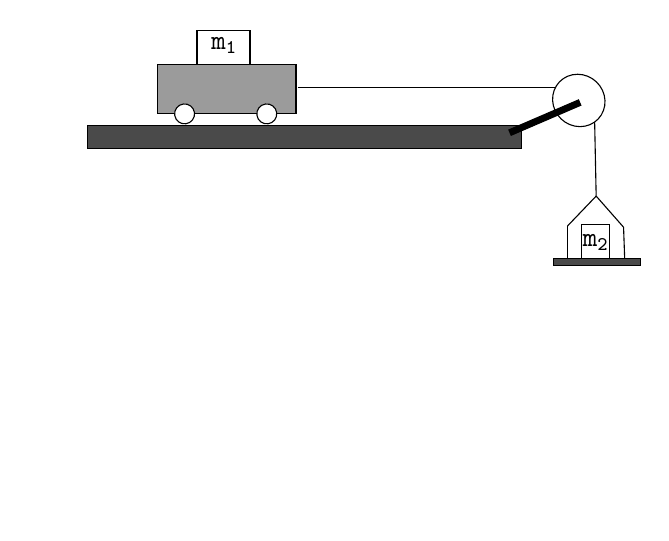
\begin{tikzpicture}[x=1pt,y=1pt,yscale=-.45,xscale=.45]
uncomment if require: \path (0,520); %set diagram left start at 0, and has height of 342

%Shape: Rectangle [id:dp2752423080869326] 
\draw  [fill={rgb, 255:red, 255; green, 255; blue, 255 }  ,fill opacity=1 ] (445,289) -- (467.5,289) -- (467.5,317) -- (445,317) -- cycle ;
%Straight Lines [id:da16986967945010711] 
\draw    (455,193) -- (455.66,225.06) -- (456.5,266) ;
%Straight Lines [id:da8918303868939179] 
\draw    (217,179) -- (441.5,179) ;
%Shape: Circle [id:dp3427863737567005] 
\draw  [fill={rgb, 255:red, 255; green, 255; blue, 255 }  ,fill opacity=1 ] (421.52,189.21) .. controls (420.97,177.59) and (429.94,168.18) .. (441.56,168.18) .. controls (453.17,168.18) and (463.03,177.59) .. (463.58,189.21) .. controls (464.13,200.82) and (455.16,210.24) .. (443.54,210.24) .. controls (431.92,210.24) and (422.06,200.82) .. (421.52,189.21) -- cycle ;
%Shape: Rectangle [id:dp2563039452319553] 
\draw  [fill={rgb, 255:red, 255; green, 255; blue, 255 }  ,fill opacity=1 ] (136,133) -- (178.5,133) -- (178.5,173) -- (136,173) -- cycle ;
%Shape: Rectangle [id:dp6528040071585879] 
\draw  [fill={rgb, 255:red, 155; green, 155; blue, 155 }  ,fill opacity=1 ] (104,160) -- (215.5,160) -- (215.5,200) -- (104,200) -- cycle ;
%Shape: Rectangle [id:dp5096708105633165] 
\draw  [fill={rgb, 255:red, 74; green, 74; blue, 74 }  ,fill opacity=1 ] (48,209) -- (396.5,209) -- (396.5,228) -- (48,228) -- cycle ;
%Shape: Circle [id:dp8948231507635738] 
\draw  [fill={rgb, 255:red, 255; green, 255; blue, 255 }  ,fill opacity=1 ] (118.08,201.1) .. controls (117.47,196.72) and (120.53,192.68) .. (124.9,192.08) .. controls (129.28,191.47) and (133.32,194.53) .. (133.92,198.9) .. controls (134.53,203.28) and (131.47,207.32) .. (127.1,207.92) .. controls (122.72,208.53) and (118.68,205.47) .. (118.08,201.1) -- cycle ;
%Shape: Circle [id:dp5290313769881847] 
\draw  [fill={rgb, 255:red, 255; green, 255; blue, 255 }  ,fill opacity=1 ] (184.08,201.1) .. controls (183.47,196.72) and (186.53,192.68) .. (190.9,192.08) .. controls (195.28,191.47) and (199.32,194.53) .. (199.92,198.9) .. controls (200.53,203.28) and (197.47,207.32) .. (193.1,207.92) .. controls (188.72,208.53) and (184.68,205.47) .. (184.08,201.1) -- cycle ;
%Shape: Rectangle [id:dp2543805907433003] 
\draw  [fill={rgb, 255:red, 0; green, 0; blue, 0 }  ,fill opacity=1 ] (386.43,212.86) -- (442.33,188.78) -- (444.17,193.05) -- (388.26,217.13) -- cycle ;
%Straight Lines [id:da16629286058204573] 
\draw    (456.5,266) -- (478.5,291) ;
%Straight Lines [id:da9603781973504766] 
\draw    (456.5,266) -- (433.5,290) ;
%Straight Lines [id:da25211031294086816] 
\draw    (433.5,290) -- (433.5,316) ;
%Straight Lines [id:da18776153488057812] 
\draw    (478.5,291) -- (479.5,319) ;
%Shape: Rectangle [id:dp647422310367781] 
\draw  [fill={rgb, 255:red, 74; green, 74; blue, 74 }  ,fill opacity=1 ] (422,316) -- (492,316) -- (492,322) -- (422,322) -- cycle ;

% Text Node
\draw (158,145) node   [align=left] { m\textsubscript{1}};
% Text Node
\draw (456.25,303) node   [align=left] { m\textsubscript{2}};
\end{tikzpicture}
\end{minipage}
\end{figure}

\newpage

\flushleft{3. Consider the same block hanging vertically and, this time, attached by a cord and pulley to a wheel having uniform mass of .1[$kg$] and a radius of .1[$m$]. Calculate the time it will take for the object to strike the ground once it is released. Hint: Keep the Moment of Inertia as the variable $I$ throughout the calculations for simplicity.\\
\vspace{24pt}
\textit{(moment of inertia for disk = $\frac{1}{2}m_dr^2$)}}

\vspace{92pt}

\begin{figure}[ht]
\begin{minipage}[b]{0.45\linewidth}
\vspace{36pt}
First, set up force equations\\\\
Bucket: $F_g - F_T = m_ba$\\
Disk: $\Sigma \tau = I \alpha$\\
\\
Then, simplify the Disk formula:
$$\cancel{r}F_T=\frac{1}{2}m_d\\r^{\cancel{2}}\\\frac{a}{\cancel{r}}$$
When substituted:
$$m_bg-\frac{1}{2}m_da=m_ba$$
When solved, $a$ is found to be:
$$a = 7.355[\si{\frac{\meter}{\square\second}}]$$
This $a$ can then be used to find $t$:\\
$$t=\sqrt{\frac{2}{a}}=.5215[\si{\second}]$$
\vspace{36pt}
\end{minipage}
\hfill\vline\hfill
\begin{minipage}[b]{0.45\linewidth}
\centering
\tikzset{every picture/.style={line width=1pt}} %set default line width to 0.75pt        

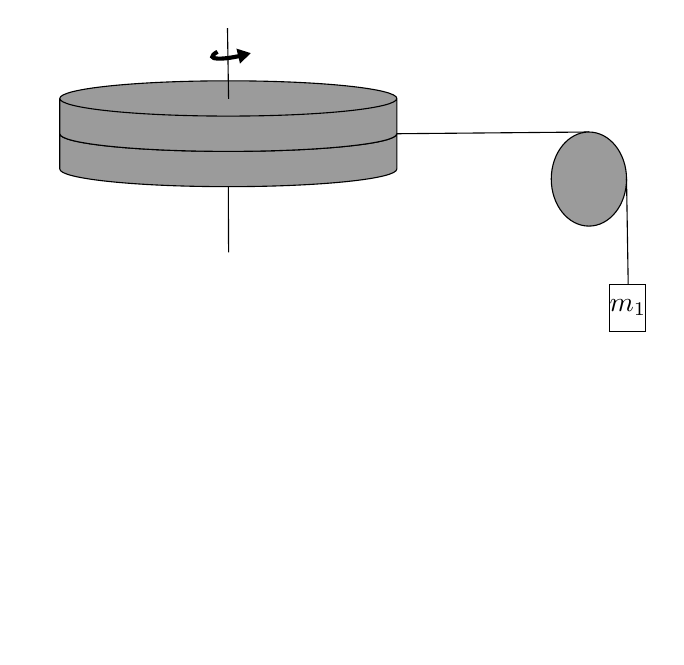
\begin{tikzpicture}[x=0.4pt,y=0.5pt,yscale=-1,xscale=1]
uncomment if require: \path (20,500); %set diagram left start at 0, and has height of 300

%Shape: Can [id:dp25019788837926127] 
\draw  [fill={rgb, 255:red, 155; green, 155; blue, 155 }  ,fill opacity=1 ] (49,136.25) -- (49,161.75) .. controls (49,168.79) and (117.16,174.5) .. (201.25,174.5) .. controls (285.34,174.5) and (353.5,168.79) .. (353.5,161.75) -- (353.5,136.25) .. controls (353.5,129.21) and (285.34,123.5) .. (201.25,123.5) .. controls (117.16,123.5) and (49,129.21) .. (49,136.25) .. controls (49,143.29) and (117.16,149) .. (201.25,149) .. controls (285.34,149) and (353.5,143.29) .. (353.5,136.25) ;
%Shape: Can [id:dp4815418998455019] 
\draw  [fill={rgb, 255:red, 155; green, 155; blue, 155 }  ,fill opacity=1 ] (49,110.75) -- (49,136.25) .. controls (49,143.29) and (117.16,149) .. (201.25,149) .. controls (285.34,149) and (353.5,143.29) .. (353.5,136.25) -- (353.5,110.75) .. controls (353.5,103.71) and (285.34,98) .. (201.25,98) .. controls (117.16,98) and (49,103.71) .. (49,110.75) .. controls (49,117.79) and (117.16,123.5) .. (201.25,123.5) .. controls (285.34,123.5) and (353.5,117.79) .. (353.5,110.75) ;

%Straight Lines [id:da6168545659537237] 
\draw    (200.5,60) -- (201.5,111) ;
%Curve Lines [id:da7173927989401014] 
\draw [line width=1.5]    (191.5,77) .. controls (177.4,83.58) and (197.76,83.09) .. (217.7,78.86) ;
\draw [shift={(221.5,78)}, rotate = 526.61] [fill={rgb, 255:red, 0; green, 0; blue, 0 }  ][line width=0.08]  [draw opacity=0] (11.61,-5.58) -- (0,0) -- (11.61,5.58) -- cycle    ;

%Straight Lines [id:da7966798261189474] 
\draw    (201.25,174.5) -- (201.5,222) ;
%Straight Lines [id:da11627198057813914] 
\draw    (353.5,136.25) -- (527,135) ;
%Shape: Circle [id:dp9162677808923885] 
\draw  [fill={rgb, 255:red, 155; green, 155; blue, 155 }  ,fill opacity=1 ] (493,169) .. controls (493,150.22) and (508.22,135) .. (527,135) .. controls (545.78,135) and (561,150.22) .. (561,169) .. controls (561,187.78) and (545.78,203) .. (527,203) .. controls (508.22,203) and (493,187.78) .. (493,169) -- cycle ;
%Straight Lines [id:da008981580424689106] 
\draw    (561,169) -- (562.5,245) ;
%Shape: Rectangle [id:dp014491786907144588] 
\draw   (546,245) -- (578.5,245) -- (578.5,279) -- (546,279) -- cycle ;

% Text Node
\draw (562.25,262) node   [align=left] {$m_1$};
\end{tikzpicture}
\end{minipage}
\end{figure}



\newpage
\section{Collected Data \& Formulas}
\vspace{24pt}
\begin{center}
\large \begin{tabular}{|l|c|c|c|c|c|}
\hline
Wheel \# & Time Trial 1 & Time Trial 2 & Time Trial 3 & Average Time \\
\hline
Wheel 1 & 4.61[$\si{\second}$] & 4.615[$\si{\second}$] & 4.31[$\si{\second}$] & 4.572[$\si{\second}$]\\
\hline
Wheel 2 & 2.79[$\si{\second}$] & 2.735[$\si{\second}$] & 2.535[$\si{\second}$] & 2.687[$\si{\second}$]\\
\hline
Wheel 3 & 1.45[$\si{\second}$] & 1.565[$\si{\second}$] & 1.565[$\si{\second}$] & 1.527[$\si{\second}$]\\
\hline
Wheel 4 & .84[$\si{\second}$] & .98[$\si{\second}$] & .805[$\si{\second}$] & .875[$\si{\second}$]\\
\hline
\end{tabular}

\large
\vspace{24pt}
\begin{tabular}{|l|c|}
\hline
    Value & Equation \\
    \hline
    Acceleration of Free Falling Mass & $g$\\
    \hline
    Angular Acceleration of the Wheel & $\alpha = \frac{a}{r}$\\
    \hline
    Final Angular Velocity of the Wheel & $\omega_f = \omega_o+\alpha t$\\
    \hline
    Moment of Inertia of the Wheel & $I =\frac{ \Sigma \tau}{\alpha}$\\
    \hline
    Angular Momentum of the Wheel & $L=I\omega$\\
    \hline
\end{tabular}

\end{center}
\vspace{24pt}
\section{Calculations\protect\footnote{Calculations performed with Wheel 3 Data}}
\subsection{Acceleration of Falling Mass}
$$v = \frac{\Delta d}{t} \longrightarrow \frac{1[\si{\meter}]}{1.527[\si{\second}]} \longrightarrow .6549 \left[ \si{\frac{\meter}{\second}} \right]$$\\
$$a = \frac{\Delta v}{t}\longrightarrow \frac{.6549 \left[ \si{\frac{\meter}{\second}} \right]}{1.527[\si{\second}]}=.4289\left[\si{\frac{\meter}{\square\second}}\right]$$

\subsection{Angular Acceleration of the Wheel}

$$a = r \alpha \longrightarrow \frac{a}{r} = \alpha$$
$$r = .0333[\si{\meter}] \longrightarrow \frac{.4289[\si{\frac{\meter}{\square\second}}]}{.0333[\si{\meter}]}$$
$$\therefore \alpha = 12.88\left[\si{\frac{\radian}{\square\second}}\right]$$
\subsection{Final Angular Velocity of the Wheel}

$$\omega_f=\omega_o+\alpha t\longrightarrow \omega_o = 0 \longrightarrow w_f=\alpha t$$
$$\omega_f=12.88\left[\si{\frac{\radian}{\square\second}}\right]*1.527[\si{\second}]\longrightarrow 19.668\left[\si{\frac{\radian}{\second}}\right]$$

\subsection{Moment of Inertia of the Wheel}

$$I = \frac{\Sigma \tau}{\alpha}\longrightarrow I = \frac{rF_T \sin(\theta)}{\alpha}$$
$$\frac{rF_T\cancel{\sin(\theta)}}{\alpha}\longrightarrow\frac{.0333[\si{\meter}]*F_T}{12.88[\frac{\si{\radian}}{\si{\square\second}}]}$$
$$F_g-F_T=ma\longrightarrow F_T=mg-ma\longrightarrow F_T=.05601[\si{\newton}]$$
$$\frac{.0333[\si{\meter}]*.05601[\si{\newton}]}{12.88[\frac{\si{\radian}}{\si{\square\second}}]}\longrightarrow .000145[\si{\kilo\gram\cdot\square\meter}]$$

\subsection{Angular Momentum of the Wheel}

$$L = I\omega \longrightarrow L = .000145[\si{\kilo\gram\cdot\square\meter}] * 19.668\left[\si{\frac{\radian}{\second}}\right]$$

$$\therefore L = .002848\left[\si{\frac{\kilo\gram\cdot\square\meter}{\second}}\right]$$



\section{Analysis}

\subsection{Data Table}
\begin{center}
\begin{tabular}{|c|c|c|c|c|c|c|c|}
\hline
& Radius & Avg. & Accel. & Angul. & Angul. & Moment of & Angul.\\ 
Wheel & $[\si{\meter}]$  & Time & of Mass & Accel. & Vel. & Inertia & Momen.
 & & &  [$\si{\second}$] &  $\left[\si{\frac{\meter}{\square\second}} \right]$ &  $\left[\si{\frac{\radian}{\square\second}} \right]$ & $\left[\si{\frac{\radian}{\second}}\right]$ & [$\si{\kilo\gram\cdot\square\meter}$] & $\left[\si{\frac{\kilogram\cdot\square\meter}{\second}}\right]$\\
 \hline
    1 & .0175 & 4.572 & .04789 & 2.733 & 12.4984 & $3.59 \cdot 10^{-4}$ & $4.482 \cdot 10^{-3}$\\
    \hline
    2 & .0250 & 2.687 & .1385 & 5.5401 & 14.887 & $2.53 \cdot 10^{-4}$ & $3.763 \cdot 10^{-3}$\\
    \hline
    3 & .0333 & 1.527 & .4289 & 12.88 & 19.668 & $1.45 \cdot 10^{-4}$ & $2.848 \cdot 10^{-3}$\\
    \hline
    4 & .0521 & .875 & 1.3061 & 25.0695 & 21.9358 & $1.16 \cdot 10^{-4}$ & $2.553 \cdot 10^{-3}$\\
    \hline
\end{tabular}
\end{center}
\subsection{Analysis Questions}

\begin{enumerate}
    
\item Explain the relationship between the radius and free fall time using words.\\
\vspace{10pt}

Free fall time is directly proportional to the square of radius. In other words, radius is inversely proportional to the square root of free fall time.
\vspace{24pt}
\item What would you expect to observe if your changing variable was the hanging mass instead of the radius of the wheel? Explain your answer using words and equations.\\
\vspace{10pt}

If the changing variable was the hanging mass, the result of increasing the mass would most likely be a decrease in time and moment of inertia, but an increase in all other factors, such as acceleration, angular velocity, and angular momentum. This is clear because the time it would take to fall would decrease, and acceleration would increase because:\\
$$v = \frac{\Delta x}{t} \rightarrow a = \frac{\Delta v}{t}$$\\
Acceleration is inversely proportional to time, and, as such, acceleration will increase because time decreases. Furthermore, angular acceleration will increase because:\\
$$\frac{a}{r}=\alpha$$\\
Because angular acceleration will increase, the moment of inertia will decrease because it is inversely proportional to angular acceleration:\\
$$I = \frac{\Sigma \tau}{\alpha}$$\\
Hence, it is clear that time and moment of inertia will decrease, whereas all other factors will increase.
\vspace{24pt}



\item What would you expect to observe if your changing variable was the mass of the rotating platform instead of the radius of the wheel? Explain your answer using words and equations.

If the mass of the rotating platform were to be increased, moment of inertia and time would increase. All other factors would decrease. This is because the force of tension is not dependent upon the mass of the platform, and is therefore constant. The formula for the moment of inertia is, with proportionality constant, $k$:\\
$$I=k*mr^2$$
With an increase in mass, the moment of inertia will be greater. Angular acceleration, and therefore all other factors, aside from time, would be less to keep proportionality:
$$\Sigma \tau = I\alpha$$
Overall, a change in platform mass would result in greater time and moment of inertia, but a decrease in all other factors.

    
\end{enumerate}
    




















\end{document}
